\section{Data and Preprocessing}
\subsection{Dataset}
The Fashion-MNIST is a dataset of Zalando article images, consisting of a training set of 60,000 samples and 10,000 test samples.
The dataset used in this project is a small subset of the original dataset consisting of 10,000 training and 5,000 test samples.
Each sample is a 28x28 pixel gray-scale image, with an associated label indicating the type of clothing.
\newline

\begin{figure}[ht]
\centering
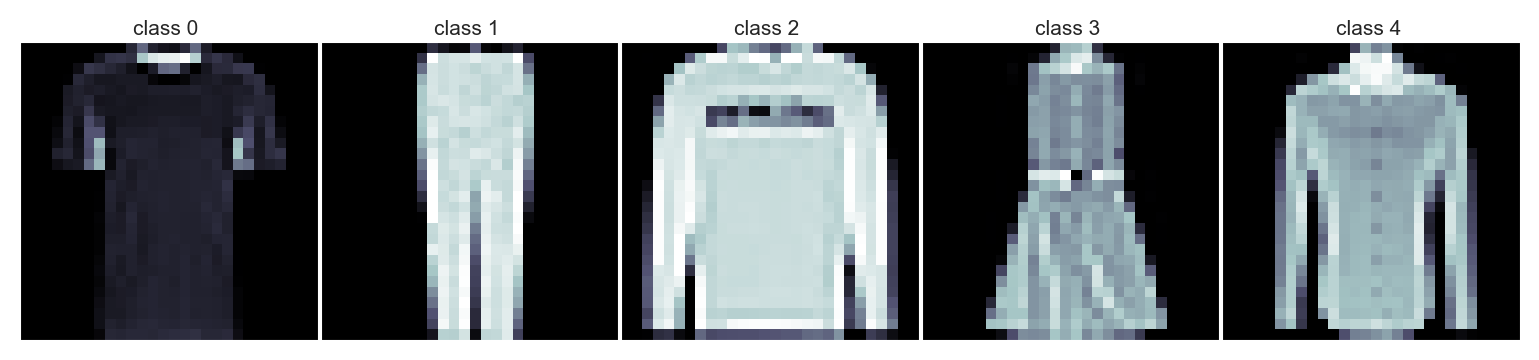
\includegraphics[scale=0.45]{figures_for_report/samples_from_classes}
\captionsetup{justification=centering,margin=2cm}
\caption{One sample from each class}
\end{figure}\\

\textbf{Table 1} shows the mapping from class label to clothing type.
The clothing types will be used instead of the labels in the report for better readability. \\
\begin{table}[H]
  \footnotesize
  \centering
\begin{tabular}{ c c c c c c }
 \toprule
 \textbf{Label} & 0 & 1 & 2 & 3 & 4 \\
 \midrule 
 \textbf{Type of clothing} & T-shirt/Top & Trousers & Pullover & Dress & Shirt \\
 \bottomrule
\end{tabular} \\[0.2cm]
\captionsetup{justification=centering,margin=2cm}
\caption{Mapping class label to clothing type}
\label{tab:features}
\end{table}


\subsection{Data Cleaning}\label{subsec:data-cleaning}
The dataset provided was already in a cleaned state, which was verified by checking for missing values,
and checking that the pixel values were no greater than 255 and no smaller than 0.

\subsection{Preprocessing}\label{subsec:preprocessing}
The pixel values were in the range $[0, 255]$.
This range was normalized to $[0, 1]$ by dividing each pixel by 255.
One reason for scaling the data is to reduce the difficulty of training a neural network, as these models can struggle to learn from large values, due to large gradient values.
Additionally, scaling the data can also slightly improve training time, as the models are able to more efficiently process smaller numbers.
\subsection{Class Distribution}\label{subsec:class-distribution}
The success of a machine learning model in predicting classes largely depends on the distribution of those classes within the training and test datasets.
Both the datasets are balanced, with the test being fully balanced ($1000$ of each class).
This is visualized in \textbf{Figure 2}.
\begin{figure}[ht]
\centering
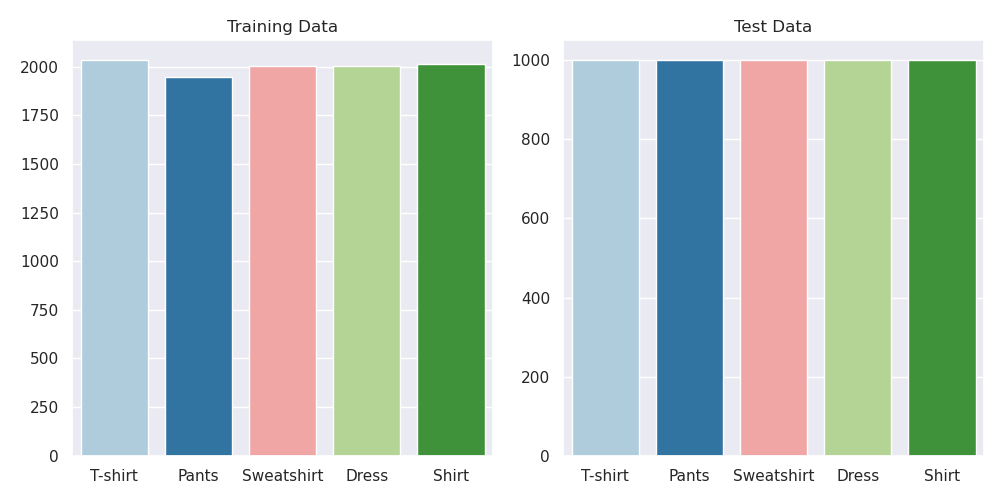
\includegraphics[scale=0.45]{figures_for_report/class_distribution}
\captionsetup{justification=centering,margin=2cm}
\caption{Distribution of clothing types in the dataset}\label{fig:figure2}
\end{figure}

